% Karrera Amarierako Proiektua egiteko LaTeX txantiloia
% itsas.ehu.es/workgroups/latex
% Unai Martinez Corral
% umartinez012@ikasle.ehu.es
%
% <- main.tex

\section{Atal bat}

\begin{figure}[!htp]
\centering
%% Karrera Amarierako Proiektua egiteko LaTeX txantiloia
% itsas.ehu.es/workgroups/latex
% Unai Martinez Corral
% umartinez012@ikasle.ehu.es
%
% <- secta_main.tex

\tikzstyle{block} = [draw, rectangle, minimum height=1cm]
\tikzstyle{sum} = [draw, circle]
\tikzstyle{inout} = [rectangle]
\tikzstyle{pinstyle} = [pin edge={to-,thin,black}]
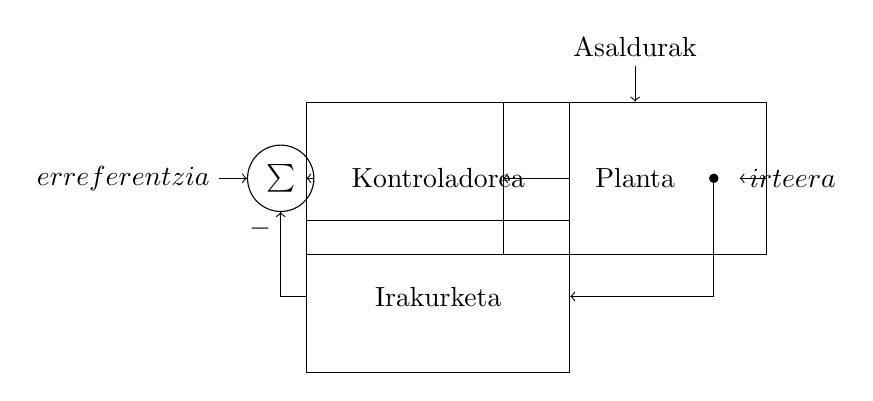
\begin{tikzpicture}[auto, node distance=1.5cm]
    \node [inout, name=input] {$erreferentzia$};
    \node [sum, right of=input,node distance=2cm] (sum) {\scriptsize $\sum$};
    \node [block, right of=sum,node distance=2cm] (controller) {Kontroladorea};
    \node [block, right of=controller, pin={[pinstyle]above:Asaldurak},
            node distance=2.5cm] (system) {Planta};
    \node [coordinate, right of=system,node distance=1cm](un){};
    \node [inout, right of=un,node distance=1cm] (output) {$irteera$};
    \node [block, below of=controller] (measurements) {Irakurketa};

    \draw [->] (input) -- node {} (sum);
    \draw [->] (sum) -- node {} (controller);
    \draw [->] (controller) -- node {} (system);
    \draw [->] (system) -- node [name=y] {} (output);
    \draw [->] (un) |- (measurements);
    \draw [->] (measurements) -| node[pos=0.9] {$-$} 
        node [near end] {} (sum);
    \draw[fill](un) circle (1.5pt);
\end{tikzpicture}

\caption{Oinarrizko berrelikatutako kontrol sistema.}
\label{fig:mod_closedloop}
\end{figure}

Ohiko berrelikatutako kontrol sistema \hyperref[fig:mod_closedloop]{\ref*{fig:mod_closedloop} irudia}n agertzen da adierazita.

\begin{equation}
\dfrac{0,94}{0,116 s + 1}
\label{eq:tf_dc}
\end{equation}

Posizio kontrola egiteko xedez, plantaren transferentzia funtzioari irabazia ($K=0.83$) eta integrazio funtzioa ($\frac{1}{s}$) biderkatu zaizkio, (\ref{eq:tf_dc_pos}) erabili da planta gisa.

\begin{equation}
\dfrac{0,94}{0,116 s + 1} \cdot {0,83} \cdot \dfrac{1}{s} = \dfrac{0,7802}{s (0,116 s + 1)}
\label{eq:tf_dc_pos}
\end{equation}

\begin{description}
\item[Proportzionala]{\hfill

Kontroladorearen sarrera den erreferentzia ($r$) eta plantaren irteeraren ($y$) arteko errore seinalea ($e$) handitu egiten du irteeran ($u$).

\[
u(t)=K_p \cdot e(t) \qquad \qquad \frac{U(s)}{E(s)}=K_d
\]}
\item[Integratzailea]{\hfill

Errore seinalea integratu eta konstante batez biderkatzen du. \emph{Automatic reset} ere esaten zaio funtzio honi.

\[
u(t)=K_i \int^t_0{e(\tau}){d\tau} \qquad \qquad \frac{U(s)}{E(s)}=\frac{K_i}{s}
\]}
\item[Deribatzailea]{\hfill

Errore seinalea deribatzen du eta konstante batez biderkatu. \emph{Anticipatory control}, \emph{rate action} edo \emph{pre-act} adierazpideak ditu.

\[
u(t)=K_d \frac{de(t)}{dt} \qquad \qquad \frac{U(s)}{E(s)}=K_d \cdot s
\]}
\end{description}

\begin{figure}[!htp]
\centering
%% Karrera Amarierako Proiektua egiteko LaTeX txantiloia
% itsas.ehu.es/workgroups/latex
% Unai Martinez Corral
% umartinez012@ikasle.ehu.es
%
% <- secta_main.tex

\begin{minipage}{.35\textwidth}
\tikzstyle{block} = [draw, rectangle, minimum height=2em, minimum width=4em]
\tikzstyle{sum} = [draw, circle]
\tikzstyle{inout} = [rectangle]
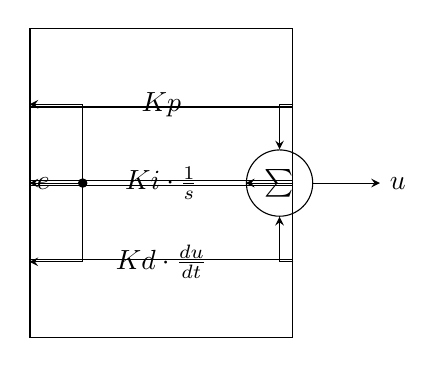
\begin{tikzpicture}[auto, node distance=1cm,>=stealth]
  \node [inout] (input) {$e$};
  \node [coordinate, right of=input,node distance=.5cm] (e) {};
  \node [block, right of=e] (int) {$Ki \cdot \frac{1}{s}$};
  \node [block, above of=int] (pro) {$Kp$};
  \node [block, below of=int] (der) {$Kd \cdot \frac{du}{dt}$};
  \node [sum, right of=int,node distance=1.5cm] (sum) {\scriptsize $\sum$};
  \node [coordinate, above of=sum] (p) {};
  \node [coordinate, below of=sum] (d) {};
  \node [inout, right of=sum,node distance=1.5cm] (output) {$u$};

  \draw [->] (input) -- (e) -- (int);
  \draw [->] (int) -- (sum);
  \draw [->] (sum) -- (output);
  \draw [->] (e) |- (pro);
  \draw [->] (pro) -- (p) -- (sum);
  \draw [->] (e) |- (der);
  \draw [->] (der) -- (d) -- (sum);
  \draw[fill](e) circle (1.5pt);
\end{tikzpicture}
\end{minipage}
\begin{minipage}{.4\textwidth}
\begin{equation}
\frac{U(s)}{E(s)} = Kp + {Ki \cdot \frac{1}{s}} + Kd \cdot s
\label{eq:cont}
\end{equation}
\vspace{.05em}
\end{minipage}

\caption[Modeloa: jarraitua (kontroladorea)]{Azterketarako erabilitako PID kontroladorearen modelo jarraitua.}
\label{fig:mod_cont_lum}
\end{figure}

\begin{figure}[!htp]
\centering
%%Anie - ohkis.sourceforge.net
%Unai Martinez Corral
%umartinez012@ikasle.ehu.es
%
% <- ./cases/anie_s3etiny_man.tex

\tikzstyle{inout} = [rectangle]
\tikzstyle{block} = [draw, rectangle, minimum height=5.5em, minimum width=9.5em]
\tikzstyle{mblock} = [draw, rectangle, minimum height=3.25em, minimum width=3.5em]
\tikzstyle{fblock} = [draw,fill=black!15, rectangle, minimum height=3.5em, minimum width=10em]
\tikzstyle{mux} = [draw, rectangle, minimum height=2.5em, minimum width=3.5em]
\tikzstyle{muxs} = [draw, rectangle, minimum height=1.5em, minimum width=3.5em]
\tikzstyle{all} = [draw, rectangle, minimum height=23em, minimum width=32em]
\tikzstyle{log} = [draw, circle, fill=gray!50,gray!50, minimum width=2em]

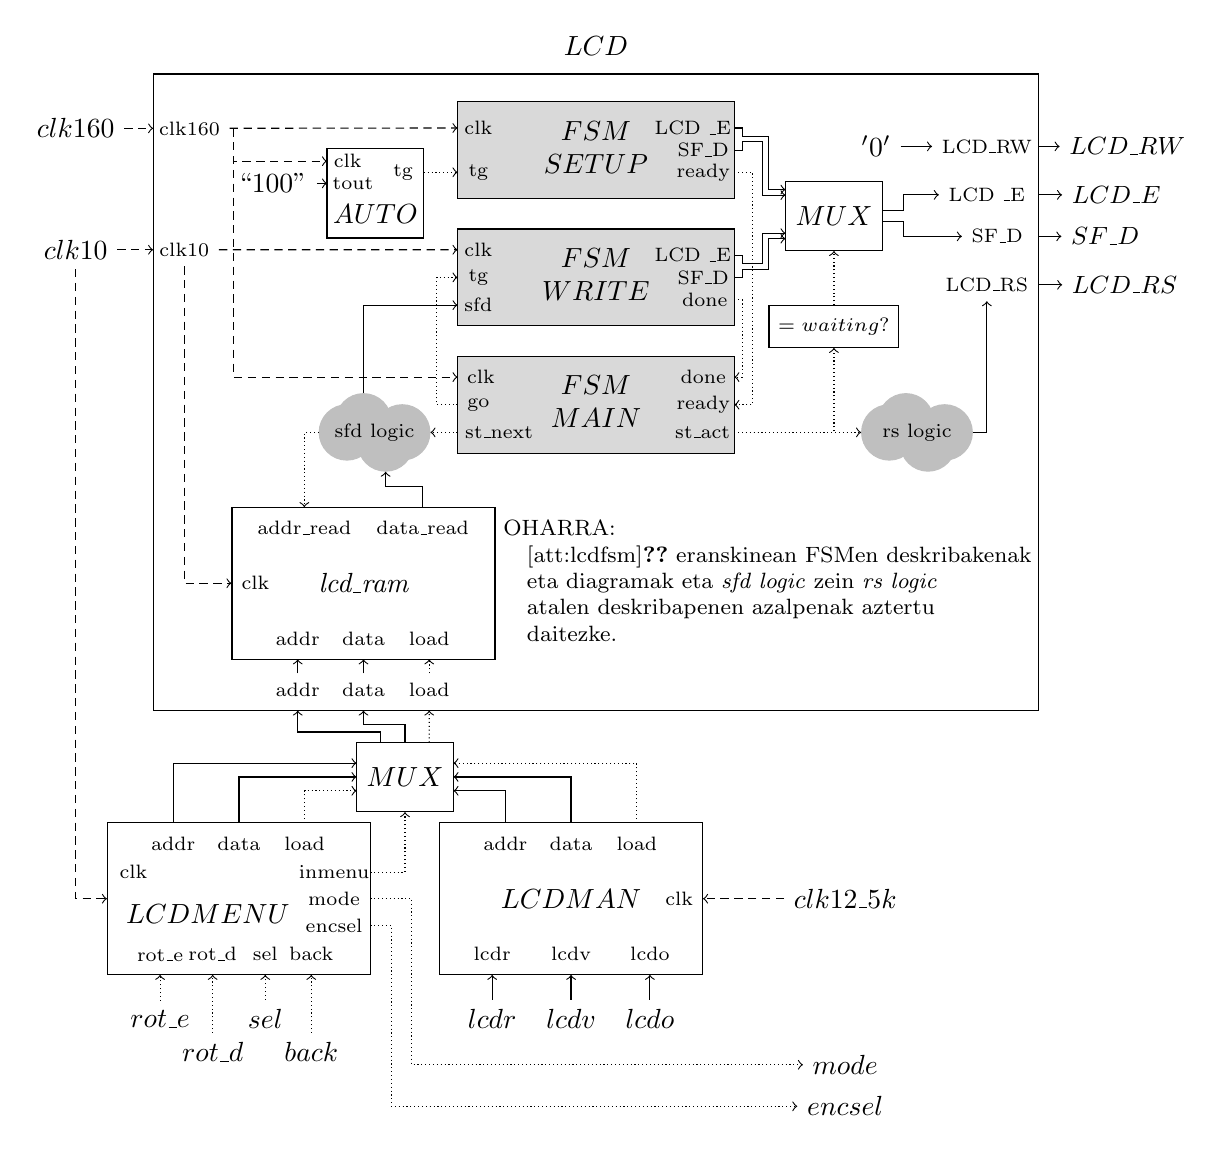
\begin{tikzpicture}[auto, node distance=5em]
 \def\sep{8em}
 \def\sepl{.75em} 
 \def\bh{2.75em}
 \def\bw{4.75em}
 \def\bhm{1em}
 \def\bwm{1.75em}
 \def\bhf{2em}
 \def\bwf{5em}
 \def\bha{11.5em}
 \def\bwa{16em}

%% LCD

  \node[all](lcd){};
  \node[inout,above of=lcd,node distance=\bha+1em](lcdl){$LCD$};
  \node[coordinate,above of=lcd,node distance=\bha](lcdn){};
  \node[coordinate,left of=lcdn,node distance=0*\bwa](fsmp){};
  \node[coordinate,below of=lcd,node distance=\bha](lcds){};
  \node[coordinate,left of=lcds,node distance=.525*\bwa](lramp){};

%% MANMUX

  \node[coordinate,right of=lramp,node distance=2*\sepl](manmuxp){};
  \node[mux,below of=manmuxp,node distance=.3*\sep](manmux){$MUX$};
  \node[coordinate,below of=manmux,node distance=.55*\sep](manp){};

  \node[coordinate,above of=manmux,node distance=1.25em](manmuxn){};
  \node[coordinate,left of=manmuxn,node distance=.5*\bwm](manmuxnw){};
  \node[coordinate,right of=manmuxn,node distance=.5*\bwm](manmuxne){};

  \node[coordinate,right of=manmux,node distance=\bwm](manmuxe){};
  \node[coordinate,above of=manmuxe,node distance=.5*\bhm](manmuxen){};
  \node[coordinate,below of=manmuxe,node distance=.5*\bhm](manmuxes){};

  \node[coordinate,left of=manmux,node distance=\bwm](manmuxw){};
  \node[coordinate,above of=manmuxw,node distance=.5*\bhm](manmuxwn){};
  \node[coordinate,below of=manmuxw,node distance=.5*\bhm](manmuxws){};

%% LCDMAN

  \node[block,right of=manp,node distance=.75*\sep](lman){$LCDMAN$};
  \node[inout,right of=lman,node distance=\bw-1.125*\sepl](lmanclk){\scriptsize clk};

%% LCDMAN SOUTH

  \node[coordinate,below of=lman,node distance=\bh](lmans){};
  \node[coordinate,left of=lmans,node distance=.6*\bw](lmansw){};
  \node[coordinate,right of=lmans,node distance=.6*\bw](lmanse){};
  \node[inout,above of=lmansw,node distance=\sepl](lref){\scriptsize lcdr};
  \node[inout,above of=lmans,node distance=\sepl](lvar){\scriptsize lcdv};
  \node[inout,above of=lmanse,node distance=\sepl](lout){\scriptsize lcdo};
  \node[inout,below of=lmansw,node distance=.2*\sep](pidref){$lcdr$};
  \node[inout,below of=lmans,node distance=.2*\sep](pidvar){$lcdv$};
  \node[inout,below of=lmanse,node distance=.2*\sep](pidout){$lcdo$};

  \draw [->] (pidref) -- (lmansw);
  \draw [->] (pidvar) -- (lmans);
  \draw [->] (pidout) -- (lmanse);

%% LCDMAN NORTH

  \node[coordinate,above of=lman,node distance=\bh](lmann){};
  \node[coordinate,left of=lmann,node distance=.5*\bw](lmannw){};
  \node[coordinate,right of=lmann,node distance=.5*\bw](lmanne){};
  \node[inout,below of=lmannw,node distance=\sepl](lmanaddr){\scriptsize addr};
  \node[inout,below of=lmann,node distance=\sepl](lmandata){\scriptsize data};
  \node[inout,below of=lmanne,node distance=\sepl](lmanload){\scriptsize load};

%% LCDMENU
  \node[block,left of=manp,node distance=.75*\sep](lmenu){};
  \node[coordinate,left of=lmenu,node distance=1.5*\sepl](lmenulgp){};
  \node[inout,below of=lmenulgp,node distance=.75*\sepl](lmenulg){$LCDMENU$};

%% LCDMENU SOUTH

  \node[coordinate,below of=lmenu,node distance=\bh](lmenus){};
  \node[coordinate,left of=lmenus,node distance=.2*\bw](lmenusw){};
  \node[coordinate,left of=lmenus,node distance=.6*\bw](lmenusww){};
  \node[coordinate,right of=lmenus,node distance=.2*\bw](lmenuse){};
  \node[coordinate,right of=lmenus,node distance=.55*\bw](lmenusee){};
  \node[inout,above of=lmenusww,node distance=.95*\sepl](rot_e){\scriptsize rot\_e};
  \node[inout,above of=lmenusw,node distance=\sepl](rot_d){\scriptsize rot\_d};
  \node[inout,above of=lmenuse,node distance=\sepl](sel){\scriptsize sel};
  \node[inout,above of=lmenusee,node distance=\sepl](back){\scriptsize back};
  \node[inout,below of=lmenusww,node distance=.2*\sep](irot_e){$rot\_e$};
  \node[inout,below of=lmenusw,node distance=.35*\sep](irot_d){$rot\_d$};
  \node[inout,below of=lmenuse,node distance=.2*\sep](isel){$sel$};
  \node[inout,below of=lmenusee,node distance=.35*\sep](iback){$back$};

  \draw [->,densely dotted] (irot_e) -- (lmenusww);
  \draw [->,densely dotted] (irot_d) -- (lmenusw);
  \draw [->,densely dotted] (isel) -- (lmenuse);
  \draw [->,densely dotted] (iback) -- (lmenusee);

%% LCDMENU NORTH

  \node[coordinate,above of=lmenu,node distance=\bh](lmenun){};
  \node[coordinate,left of=lmenun,node distance=.5*\bw](lmenunw){};
  \node[coordinate,right of=lmenun,node distance=.5*\bw](lmenune){};
  \node[inout,below of=lmenunw,node distance=\sepl](lmenuaddr){\scriptsize addr};
  \node[inout,below of=lmenun,node distance=\sepl](lmenudata){\scriptsize data};
  \node[inout,below of=lmenune,node distance=\sepl](lmenuload){\scriptsize load};

%% LCDMENU EAST

  \node[coordinate,right of=lmenu,node distance=\bw](lmenue){};
  \node[coordinate,above of=lmenue,node distance=.35*\bh](lmenuen){};
  \node[coordinate,below of=lmenue,node distance=.35*\bh](lmenues){};
  \node[inout,left of=lmenuen,node distance=1.75*\sepl](lmenuin){\scriptsize inmenu};
  \node[inout,left of=lmenue,node distance=1.75*\sepl](lmenumode){\scriptsize mode};
  \node[inout,left of=lmenues,node distance=1.75*\sepl](lmenuencsel){\scriptsize encsel};

  \draw[->,densely dotted](lmenuen) -| (manmux);

  \node[coordinate,right of=lmenue,node distance=2*\sepl](lmenue_r){};
  \node[coordinate,right of=lmenues,node distance=1*\sepl](lmenues_r){};

%% LCDMENU WEST

  \node[coordinate,left of=lmenu,node distance=\bw](lmenuw){};
  \node[coordinate,above of=lmenuw,node distance=.35*\bh](lmenuwn){};
  \node[inout,right of=lmenuwn,node distance=1.25*\sepl](lmenuinmenu){\scriptsize clk};

%% LCD SOUTH

  \node[coordinate,left of=lramp,node distance=.5*\bw](lrampw){};
  \node[coordinate,right of=lramp,node distance=.5*\bw](lrampe){};
  \node[inout,above of=lrampw,node distance=\sepl](lcdaddr){\scriptsize addr};
  \node[inout,above of=lramp,node distance=\sepl](lcddata){\scriptsize data};
  \node[inout,above of=lrampe,node distance=\sepl](lcdload){\scriptsize load};

  \node[coordinate,above of=manmuxnw,node distance=.5*\sepl](manmuxnw_a){};
  \node[coordinate,above of=manmuxn,node distance=.875*\sepl](manmuxn_a){};
  \draw [->] (manmuxnw) -- (manmuxnw_a) -| (lrampw);
  \draw [->] (manmuxn) -- (manmuxn_a) -| (lramp);
  \draw [->,densely dotted] (manmuxne)  -- (lrampe);

  \draw [->] (lmannw) |- (manmuxes);
  \draw [->] (lmann) |- (manmuxe);
  \draw [->,densely dotted] (lmanne) |- (manmuxen);

  \draw [->] (lmenunw) |- (manmuxwn);
  \draw [->] (lmenun) |- (manmuxw);
  \draw [->,densely dotted] (lmenune) |- (manmuxws);

%% LCD RAM

  \node[block,above of=lramp,node distance=.575*\sep](lram){\itshape lcd\_ram};
  \node[inout,left of=lram,node distance=\bw-1.125*\sepl](lramclk){\scriptsize clk};
  \node[coordinate,below of=lram,node distance=\bh](lrams){};
  \node[coordinate,left of=lrams,node distance=.5*\bw](lramsw){};
  \node[coordinate,right of=lrams,node distance=.5*\bw](lramse){};
  \node[inout,above of=lramsw,node distance=\sepl](lramaddr){\scriptsize addr};
  \node[inout,above of=lrams,node distance=\sepl](lramdata){\scriptsize data};
  \node[inout,above of=lramse,node distance=\sepl](lramload){\scriptsize load};
  \node[coordinate,above of=lram,node distance=\bh](lramn){};
  \node[coordinate,left of=lramn,node distance=.45*\bw](lramnw){};
  \node[coordinate,right of=lramn,node distance=.45*\bw](lramne){};
  \node[inout,below of=lramnw,node distance=\sepl](lramaddrr){\scriptsize addr\_read};
  \node[inout,below of=lramne,node distance=\sepl](lcdramdatar){\scriptsize data\_read};

  \draw [->] (lcdaddr) -- (lramsw);
  \draw [->] (lcddata) -- (lrams);
  \draw [->,densely dotted] (lcdload) -- (lramse);

  \node[coordinate,left of=lram,node distance=\bw+\sepl](lram_l){};

%% FSM_SETUP

  \node[fblock,below of=fsmp,node distance=\sepl+\bhf](lsetup){\begin{tabular}{c}$FSM$\\$SETUP$\end{tabular}};
  \node[coordinate,right of=lsetup,node distance=\bwf](lsetupe){};
  \node[coordinate,above of=lsetupe,node distance=.4*\bhf](lsetupen){};
  \node[coordinate,below of=lsetupe,node distance=.4*\bhf](lsetupes){};
  \node[inout,left of=lsetupen,node distance=2*\sepl](lsetupeo){\scriptsize LCD \_E};
  \node[inout,left of=lsetupe,node distance=1.5*\sepl](lsetupsfd){\scriptsize SF\_D};
  \node[inout,left of=lsetupes,node distance=1.5*\sepl](lsetupready){\scriptsize ready};
  \node[coordinate,left of=lsetup,node distance=\bwf](lsetupw){};
  \node[coordinate,above of=lsetupw,node distance=.4*\bhf](lsetupwn){};
  \node[coordinate,below of=lsetupw,node distance=.4*\bhf](lsetupws){};
  \node[inout,right of=lsetupwn,node distance=\sepl](lsetupclk){\scriptsize clk};
  \node[inout,right of=lsetupws,node distance=\sepl](lsetuptg){\scriptsize tg};

%% FSM_WRITE

  \node[fblock,below of=lsetup,node distance=.575*\sep](lwrite){\begin{tabular}{c}$FSM$\\$WRITE$\end{tabular}};
  \node[coordinate,right of=lwrite,node distance=\bwf](lwritee){};
  \node[coordinate,above of=lwritee,node distance=.4*\bhf](lwriteen){};
  \node[coordinate,below of=lwritee,node distance=.4*\bhf](lwritees){};
  \node[inout,left of=lwriteen,node distance=2*\sepl](lwriteeo){\scriptsize LCD \_E};
  \node[inout,left of=lwritee,node distance=1.5*\sepl](lwritesfd){\scriptsize SF\_D};
  \node[inout,left of=lwritees,node distance=1.425*\sepl](lwritedone){\scriptsize done};
  \node[coordinate,left of=lwrite,node distance=\bwf](lwritew){};
  \node[coordinate,above of=lwritew,node distance=.5*\bhf](lwritewn){};
  \node[coordinate,below of=lwritew,node distance=.5*\bhf](lwritews){};
  \node[inout,right of=lwritewn,node distance=\sepl](lwriteclk){\scriptsize clk};
  \node[inout,right of=lwritew,node distance=\sepl](lwritetg){\scriptsize tg};
  \node[inout,right of=lwritews,node distance=\sepl](lwritesfd){\scriptsize sfd};

%% FSM_MAIN

  \node[fblock,below of=lwrite,node distance=.575*\sep](lmain){\begin{tabular}{c}$FSM$\\$MAIN$\end{tabular}};
  \node[coordinate,left of=lmain,node distance=\bwf](lmainw){};
  \node[coordinate,above of=lmainw,node distance=.5*\bhf](lmainwn){};
  \node[coordinate,below of=lmainw,node distance=.5*\bhf](lmainws){};
  \node[inout,right of=lmainwn,node distance=1.125*\sepl](lmainclk){\scriptsize clk};
  \node[inout,right of=lmainw,node distance=1*\sepl](lmainclk){\scriptsize go};
  \node[inout,right of=lmainws,node distance=2*\sepl](lmainst){\scriptsize st\_next};
  \node[coordinate,right of=lmain,node distance=\bwf](lmaine){};
  \node[coordinate,below of=lmaine,node distance=.5*\bhf](lmaines){};
  \node[inout,left of=lmaines,node distance=1.525*\sepl](lmainst){\scriptsize st\_act};
  \node[coordinate,above of=lmaine,node distance=.5*\bhf](lmainen){};
  \node[inout,left of=lmaine,node distance=1.5*\sepl](lmainready){\scriptsize ready};
  \node[inout,left of=lmainen,node distance=1.5*\sepl](lmaindone){\scriptsize done};

  \node[coordinate,left of=lmainw,node distance=\sepl](lmainw_l){};
  \draw [->,densely dotted] (lmainw) -- (lmainw_l) |- (lwritew);

%% LCDAUTO

  \node[coordinate,left of=lsetupws,node distance=.625*\bw](lauto_p){};
  \node[mblock,below of=lauto_p,node distance=.75*\bhm](lauto){};
  \node[inout,below of=lauto,node distance=.75*\bhm](lautol){$AUTO$};
  \node[coordinate,above of=lauto,node distance=.75*\bhm](lautor){};
  \node[coordinate,left of=lautor,node distance=\bwm](lautow){};
  \node[coordinate,above of=lautow,node distance=.4*\bhm](lautown){};
  \node[coordinate,below of=lautow,node distance=.4*\bhm](lautows){};
  \node[inout,right of=lautown,node distance=\sepl](lautoclk){\scriptsize clk};
  \node[inout,right of=lautows,node distance=1.25*\sepl](lautotout){\scriptsize tout};
  \node[inout,left of=lautows,node distance=1.125*\bwm](tout){$``100"$};
  \draw [->] (tout) -- (lautows);
  \node[coordinate,right of=lautor,node distance=\bwm](lautoe){};
  \node[inout,left of=lautoe,node distance=\sepl](lautotg){\scriptsize tg};
  \draw [->,densely dotted] (lautoe) -- (lsetupws);

%% MUX

  \node [coordinate,right of=lsetupen,node distance=.375*\sepl](lsetupen_r){};
  \node [coordinate,below of=lsetupen_r,node distance=.15*\bhf](lsetupen_rb){};
  \node [coordinate,right of=lsetupe,node distance=.375*\sepl](lsetupe_r){};
  \node [coordinate,above of=lsetupe_r,node distance=.15*\bhf](lsetupe_ra){};
  \node [coordinate,right of=lsetupen_rb,node distance=.375*\bhf+.1*\bhf](lsetupen_rb_r){};
  \node [coordinate,right of=lsetupe_ra,node distance=.375*\bhf](lsetupe_ra_r){};

  \node [coordinate,right of=lwriteen,node distance=.375*\sepl](lwriteen_r){};
  \node [coordinate,below of=lwriteen_r,node distance=.15*\bhf](lwriteen_rb){};
  \node [coordinate,right of=lwritee,node distance=.375*\sepl](lwritee_r){};
  \node [coordinate,above of=lwritee_r,node distance=.15*\bhf](lwritee_ra){};
  \node [coordinate,right of=lwriteen_rb,node distance=.375*\bhf](lwriteen_rb_r){};
  \node [coordinate,right of=lwritee_ra,node distance=.375*\bhf+.1*\bhf](lwritee_ra_r){};

  \node[coordinate,right of=lsetupe,node distance=.45*\sep](mux_p){};
  \node[mux,below of=mux_p,node distance=.2875*\sep+.075em](mux){$MUX$};
  \node[coordinate,right of=mux,node distance=1.75em](muxe){};
  \node[coordinate,above of=muxe,node distance=.1*\bhf](muxen){};
  \node[coordinate,below of=muxe,node distance=.1*\bhf](muxes){};

  \node [coordinate,right of=muxen,node distance=\sepl](muxen_r){};
  \node [coordinate,right of=muxes,node distance=\sepl](muxes_r){};

  \node[coordinate,left of=mux,node distance=1.75em](muxw){};
  \node[coordinate,above of=muxw,node distance=.75em](muxwn){}; 
  \node[coordinate,above of=muxwn,node distance=.1*\bhf](muxwnn){}; 
  \node[coordinate,below of=muxw,node distance=.625em](muxws){};
  \node[coordinate,below of=muxws,node distance=.1*\bhf](muxwss){}; 

  \node[coordinate,right of=lsetupes,node distance=.875*\sepl](lsetupes_r){};
  \draw [->,densely dotted] (lsetupes) -- (lsetupes_r) |- (lmaine);
  \node[coordinate,right of=lwritees,node distance=.375*\sepl](lwritees_r){};
  \draw [->,densely dotted] (lwritees) -- (lwritees_r) |- (lmainen);

  \draw [->] (lsetupen) -| (lsetupen_rb) -- (lsetupen_rb_r) |- (muxwnn);
  \draw [->] (lsetupe) -| (lsetupe_ra) -- (lsetupe_ra_r) |- (muxwn);

  \draw [->] (lwriteen) -| (lwriteen_rb) -- (lwriteen_rb_r) |- (muxws);
  \draw [->] (lwritee) -| (lwritee_ra) -- (lwritee_ra_r) |- (muxwss);

%% LCD EAST

  \node[coordinate,right of=lcd,node distance=\bwa](lcdlp){};
  \node[coordinate,above of=lcdlp,node distance=.7725*\bha](lcdl1){};
  \node[coordinate,below of=lcdl1,node distance=.875*\bhf](lcdl2){};
  \node[coordinate,below of=lcdl2,node distance=.75*\bhf](lcdl3){};
  \node[coordinate,below of=lcdl3,node distance=.875*\bhf](lcdl4){};
  \node[inout,left of=lcdl4,node distance=2.5*\sepl](lcdrs){\scriptsize LCD\_RS};
  \node[inout,left of=lcdl1,node distance=2.5*\sepl](lcdrw){\scriptsize LCD\_RW};
  \node[inout,left of=lcdl2,node distance=2.5*\sepl](lcde){\scriptsize LCD \_E};
  \node[inout,left of=lcdl3,node distance=2*\sepl](lcdsfd){\scriptsize SF\_D};

  \draw [->] (muxen) -- (muxen_r) |- (lcde);
  \draw [->] (muxes) -- (muxes_r) |- (lcdsfd);

%% MUX SEL

  \node[coordinate,below of=mux,node distance=.3*\sep](muxselp){};
  \node[muxs,below of=mux,node distance=.5*\sep](muxsel){\scriptsize $=waiting?$};
  
  \draw [->,densely dotted] (lmaines) -| (muxsel);
  \draw [->,densely dotted] (muxsel) -- (mux);
 
  \node[inout,left of=lcdrw,node distance=.5*\sep](lcdrwconst){$'0'$};
  \draw [->] (lcdrwconst) -- (lcdrw);

  \node [coordinate,below of=muxsel,node distance=.625*\sep] (logic1p) {};
  \node [coordinate,right of=lmaines,node distance=.825*\sep] (logic1) {};
  \node [log,left of=logic1,node distance=.125*\sep] (logic1w) {}; 
  \node [log,right of=logic1,node distance=.125*\sep] (logic1e) {};
  \node [coordinate,above of=logic1,node distance=.05*\sep] (logic1_a) {};
  \node [log,left of=logic1_a,node distance=.05*\sep] (logic1n){}; 
  \node [coordinate,below of=logic1,node distance=.05*\sep] (logic1_b) {};
  \node [log,right of=logic1_b,node distance=.05*\sep] (logic1s){};
  \node [inout,below of=logic1,node distance=0] {\scriptsize rs logic};
  \draw [->,densely dotted] (lmaines) -- (logic1w);
  \draw [->] (logic1e) -| (lcdrs);

  \node [coordinate,left of=lmainws,node distance=.375*\sep] (logic2) {};
  \node [log,left of=logic2,node distance=.125*\sep] (logic2w) {}; 
  \node [log,right of=logic2,node distance=.125*\sep] (logic2e) {};
  \node [coordinate,above of=logic2,node distance=.05*\sep] (logic2_a) {};
  \node [log,left of=logic2_a,node distance=.05*\sep] (logic2n){}; 
  \node [coordinate,below of=logic2,node distance=.05*\sep] (logic2_b) {};
  \node [log,right of=logic2_b,node distance=.05*\sep] (logic2s){};
  \draw [->,densely dotted] (lmainws) -- (logic2e);
  \draw [->,densely dotted] (logic2w) -| (lramnw);
  \node [coordinate,above of=lramne,node distance=\sepl](lramne_a){};
  \draw [->] (lramne) -- (lramne_a) -| (logic2s);
  \node [inout,below of=logic2,node distance=0] {\scriptsize sfd logic};

  \draw [->] (logic2n) |- (lwritews);

%% LCD WEST

  \node[coordinate,left of=lcd,node distance=\bwa](lcdw){};
  \node[coordinate,above of=lcdw,node distance=.825*\bha+.025*\bhf](lcdwn){};
  \node[coordinate,above of=lcdw,node distance=.65*\sep-.025*\bhf](lcdws){};
  \node[inout,right of=lcdwn,node distance=1.75*\sepl](lcdclk160){\scriptsize clk160};
  \node[inout,right of=lcdws,node distance=1.5*\sepl](lcdclk10){\scriptsize clk10};

%% CLK

  \node[inout,left of=lcdwn,node distance=.35*\sep](c160){$clk160$};
  \node[inout,left of=lcdws,node distance=.35*\sep](c10){$clk10$};
  \node[inout,right of=lmanclk,node distance=.75*\sep](c0_5k){$clk12\_5k$};

  \node[coordinate,right of=lcdclk160,node distance=.15*\sep](lcdclk160rp){};
  \node[coordinate,right of=lcdclk160,node distance=.2*\sep](lcdclk160_r){};

  \draw [->,densely dashed] (c160) -- (lcdwn);
  \draw [->,densely dashed] (c10) -- (lcdws);
  \draw [->,densely dashed] (c10) |- (lmenu);
  \draw [->,densely dashed] (c0_5k) -- (lman);

  \draw [->,densely dashed] (lcdclk160) -- (lsetupwn);
  \draw [->,densely dashed] (lcdclk160_r) |- (lautown);
  \draw [->,densely dashed] (lcdclk160_r) |- (lmainwn);

  \draw [->,densely dashed] (lcdclk10) -- (lwritewn);
  \draw [->,densely dashed] (lcdclk10) |- (lram);

  \node[inout,below of=c0_5k,node distance=.75*\sep](omode){$mode$};
  \node[inout,below of=omode,node distance=2*\sepl](oencsel){$encsel$};
  \draw[->,densely dotted](lmenue) -- (lmenue_r) |- (omode);
  \draw[->,densely dotted](lmenues) -- (lmenues_r) |- (oencsel);

%% OUT

  \node[inout,right of=lcdl1,node distance=.4*\sep](orw){\small $LCD\_RW$};
  \node[inout,right of=lcdl2,node distance=.35*\sep](oe){\small $LCD\_E$};
  \node[inout,right of=lcdl3,node distance=.3*\sep](osfd){\small $SF\_D$};
  \node[inout,right of=lcdl4,node distance=.3875*\sep](ors){\small $LCD\_RS$};

  \draw [->] (lcdl1) -- (orw);
  \draw [->] (lcdl2) -- (oe);
  \draw [->] (lcdl3) -- (osfd);
  \draw [->] (lcdl4) -- (ors);

  \node[inout,right of=lram,node distance=1.825*\sep](note){\footnotesize\begin{tabular}{l}
OHARRA: 
\\
\hskip 1em \hyperref[att:lcdfsm]{\ref*{att:lcdfsm} eranskin}ean FSMen deskribakenak\\
\hskip 1em eta diagramak eta \emph{sfd logic} zein \emph{rs logic}\\
\hskip 1em atalen deskribapenen azalpenak aztertu\\
\hskip 1emdaitezke.
\end{tabular}
};

\end{tikzpicture}

\caption{LCD kudeatzailea.}
\label{fig:lcd}
\end{figure}